\documentclass{article}

% Set page size and margins
\usepackage[letterpaper,top=2cm,bottom=2cm,left=3cm,right=3cm,marginparwidth=1.75cm]{geometry}

% Useful packages
\usepackage{amsmath}
\usepackage{graphicx}
\usepackage[colorlinks=true, allcolors=blue]{hyperref}

\title{0A - Stack Analysis}
\author{Jordan King}
\date{November 3, 2023}

\begin{document}
\maketitle

\section{Part A: Counting}

\begin{table}[h!]
\centering
\begin{tabular}{c|c|c|c|c|c|c|c|c|c}
Push & 1 & 2 & 3 & 4 & 5 & 6 & 7 & 8 & 9 \\\hline
Every Time Count & 1 & 1 & 1 & 1 & 1 & 1 & 1 & 1 & 1 \\
Array Copy Count & 0 & 1 & 2 & 0 & 4 & 0 & 0 & 0 & 8 \\
$C_{cumulative (n)}$ & 1 & 2 & 3 & 1 & 5 & 1 & 1 & 1 & 9
\end{tabular}
\caption{\label{tab:widgets}Pushes and resulting array assignments.}
\end{table} 

Assignments required in the worst case for a push: $O(n)$\\

When $n = 2^k + 1$, $C_{cumulative (n)} = 2n - 3$ \\ 

Sample calculation: when push $= 9$, $C_{cumulative (n)} = 15$, so $2(9) - 3 = 15$ \\

$C_{avg} = (C_{cumulative (n)}) / n = (2n - 3) / n$ \\

As n goes to infinity, $C_{avg}$ approaches a simple integer bound: \\

\[ \lim_{n\to\infty} (2n - 3) / n = 2\] \\

Thus, the average cost after many pushes is bounded by two. \\

\section{Part B: Experiments}
\subsection{Experiment 1}
In this experiment, we measure how the average time for a push changes as the number of pushes increases for two different push functions: 1) push function that doubles the array when capacity is reached and 2) push function that creates a new array at every push. \\

First, the push function that doubles the array when capacity is reached (Push1): \\

\begin{table}[h!]
\centering
\begin{tabular}{c|c|c|c|c|c|c|c|c|c|l}
Number of\\Pushes & 10000 & 20000 & 30000 & 40000 & 50000 & 60000 & 70000 & 80000 & 90000 & 100000 \\\hline
Avg Time \\Per Push (s) & 2.38E-8 & 2.27E-8 & 2.18E-8 & 2.19E-8 & 2.09E-8 & 1.77E-8 & 2.33E-8 & 2.21E-8 & 2.18E-8 & 2.17E-8 \\

\end{tabular}
\caption{\label{tab:widgets}Average time in seconds required for a push as the number of pushes changes (using push function that doubles array when capacity is reached)}
\end{table}

\pagebreak

Next, the push function that creates a new array at each push (Push2): 

\begin{table}[h!]
\centering
\begin{tabular}{c|c|c|c|c|c|c|c|c|c|l}
Number of\\Pushes & 10000 & 20000 & 30000 & 40000 & 50000 & 60000 & 70000 & 80000 & 90000 & 100000 \\\hline
Avg Time\\Per Push (s) & 1.26E-5 & 2.52E-5 & 3.74E-5 & 4.89E-5 & 6.02E-5 & 7.14E-5 & 8.41E-5 & 9.54E-5 & 1.07E-4 & 1.18E-4 \\

\end{tabular}
\caption{\label{tab:widgets}Average time in seconds required for a push as the number of pushes changes (using push function that creates a new array every push)}
\end{table}

\begin{figure}[h!]
  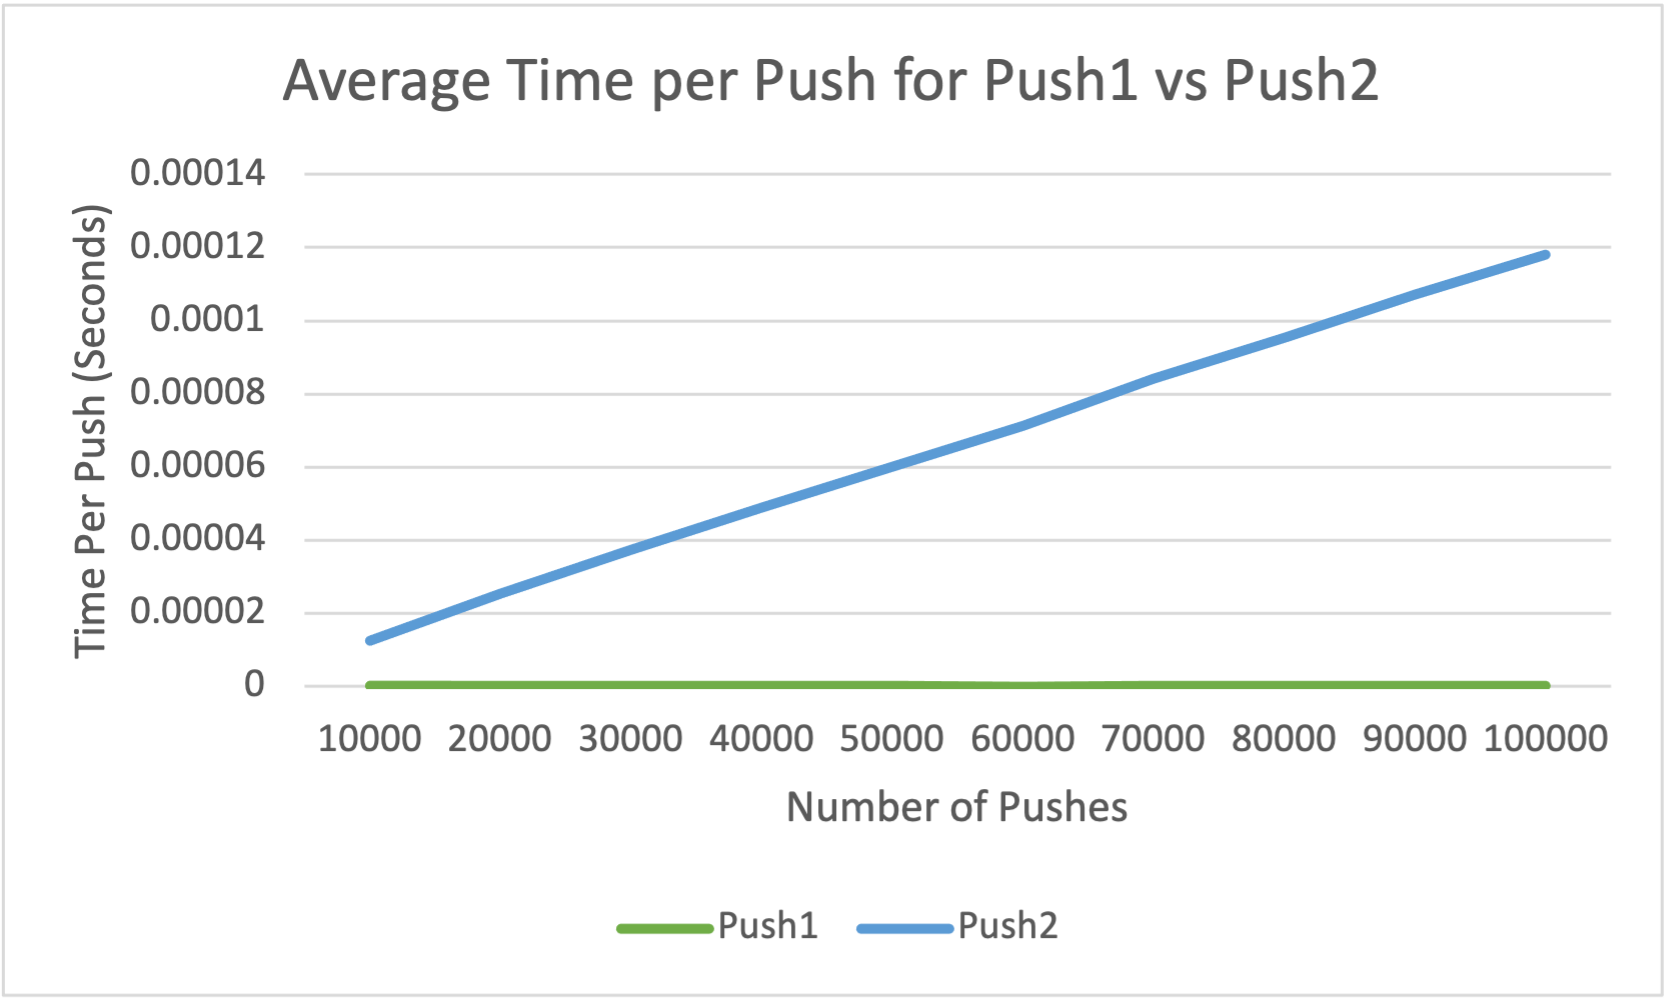
\includegraphics[width=\linewidth]{Figure1_0A.png}
  \caption{Average Time per Push for Push1 vs Push2}
  \label{fig:boat1}
\end{figure}

As seen in Figure 1, Push1, the algorithm that doubles the array once capacity is reached, is significantly faster than Push2, which increases the capacity of the array by one each time. 

\subsection{Experiment 2}

In this experiment, a push function (Push3) is created that increases the size of the array by 10 when capacity is reached, and measure how the average time for a push changes as the number of pushes increases. This will be compared to Push1. 
Hypothesis: A push function that increases the size of the array by 10 each time capacity is reached will be only slightly faster (0.5x faster) than a push function that increases the size of the array by one each time.  

\begin{table}[h!]
\centering
\begin{tabular}{c|c|c|c|c|c|c|c|c|c|l}
Number of\\Pushes & 10000 & 20000 & 30000 & 40000 & 50000 & 60000 & 70000 & 80000 & 90000 & 100000 \\\hline
Avg Time\\Per Push (s) & 1.36E-5 & 2.52E-5 & 3.89E-5 & 5.22E-5 & 6.53E-5 & 7.79E-5 & 9.22E-5 & 1.05E-4 & 1.19E-4 & 1.33E-4 \\

\end{tabular}
\caption{\label{tab:widgets}Average time in seconds required for a push as the number of pushes changes (using push function that increases capacity by 10 each push)}
\end{table}

\pagebreak

\begin{figure}[h!]
  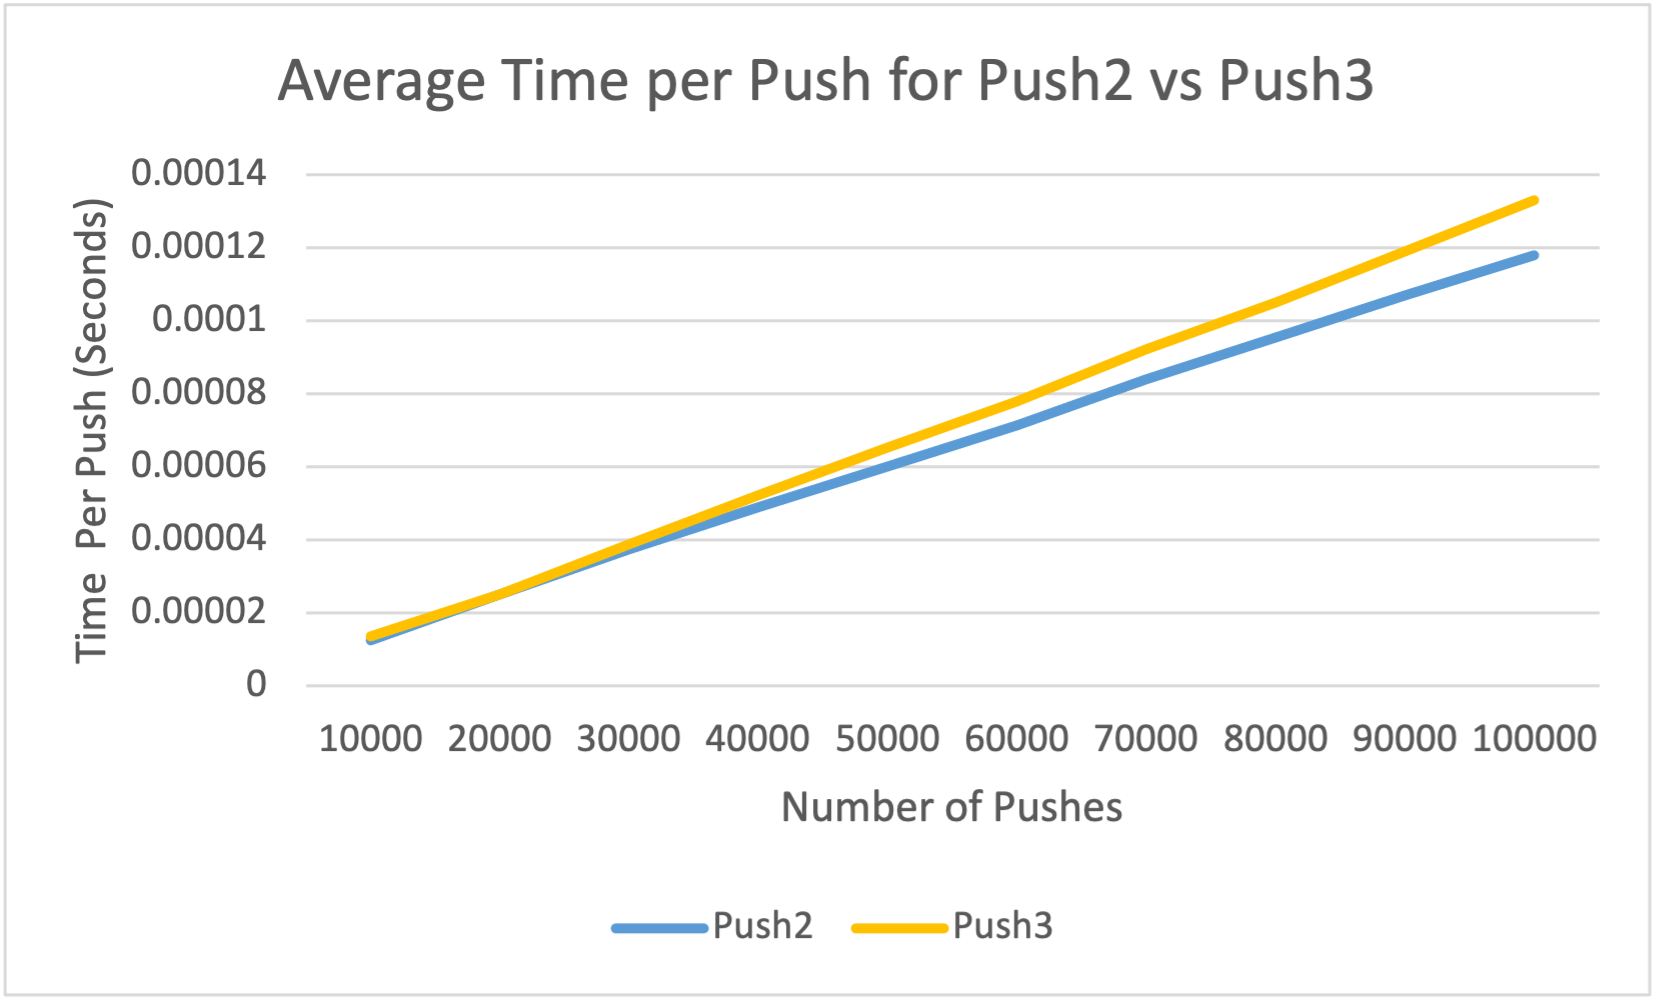
\includegraphics[width=\linewidth]{Figure2_0A.png}
  \caption{Average Time per Push for Push2 vs Push3}
  \label{fig:boat1}
\end{figure}

As shown in Figure2, Push2 and Push3 has very similar average times per push, with Push3 being a fraction of a second slower than Push1 (for example, with 100,000 pushes, the average time for a push using Push3 was 1.5E-5 seconds slower than Push2. This does not support the hypothesis that Push3 would be 0.5x faster than Push2. 
\pagebreak 

\subsection{Experiment 3}

In this experiment, a push function is created (Push4) that instead of doubling the capacity each time, the capacity is multiplied by 1.5.
Hypothesis: Push4 will be 0.5x slower than Push1.  

\begin{table}[h!]
\centering
\begin{tabular}{c|c|c|c|c|c|c|c|c|c|l}
Number of\\Pushes & 10000 & 20000 & 30000 & 40000 & 50000 & 60000 & 70000 & 80000 & 90000 & 100000 \\\hline
Avg Time\\Per Push (s) & 3.70E-8 & 3.71E-8 & 3.73E-8 & 2.77E-8 & 2.92E-8 & 3.00E-8 & 3.05E-8 & 3.13E-8 & 2.99E-8 & 3.18E-8 \\

\end{tabular}
\caption{\label{tab:widgets}Average time in seconds required for a push as the number of pushes changes (using push function that multiplies capacity by 1.5)}
\end{table}

\begin{figure}[h!]
  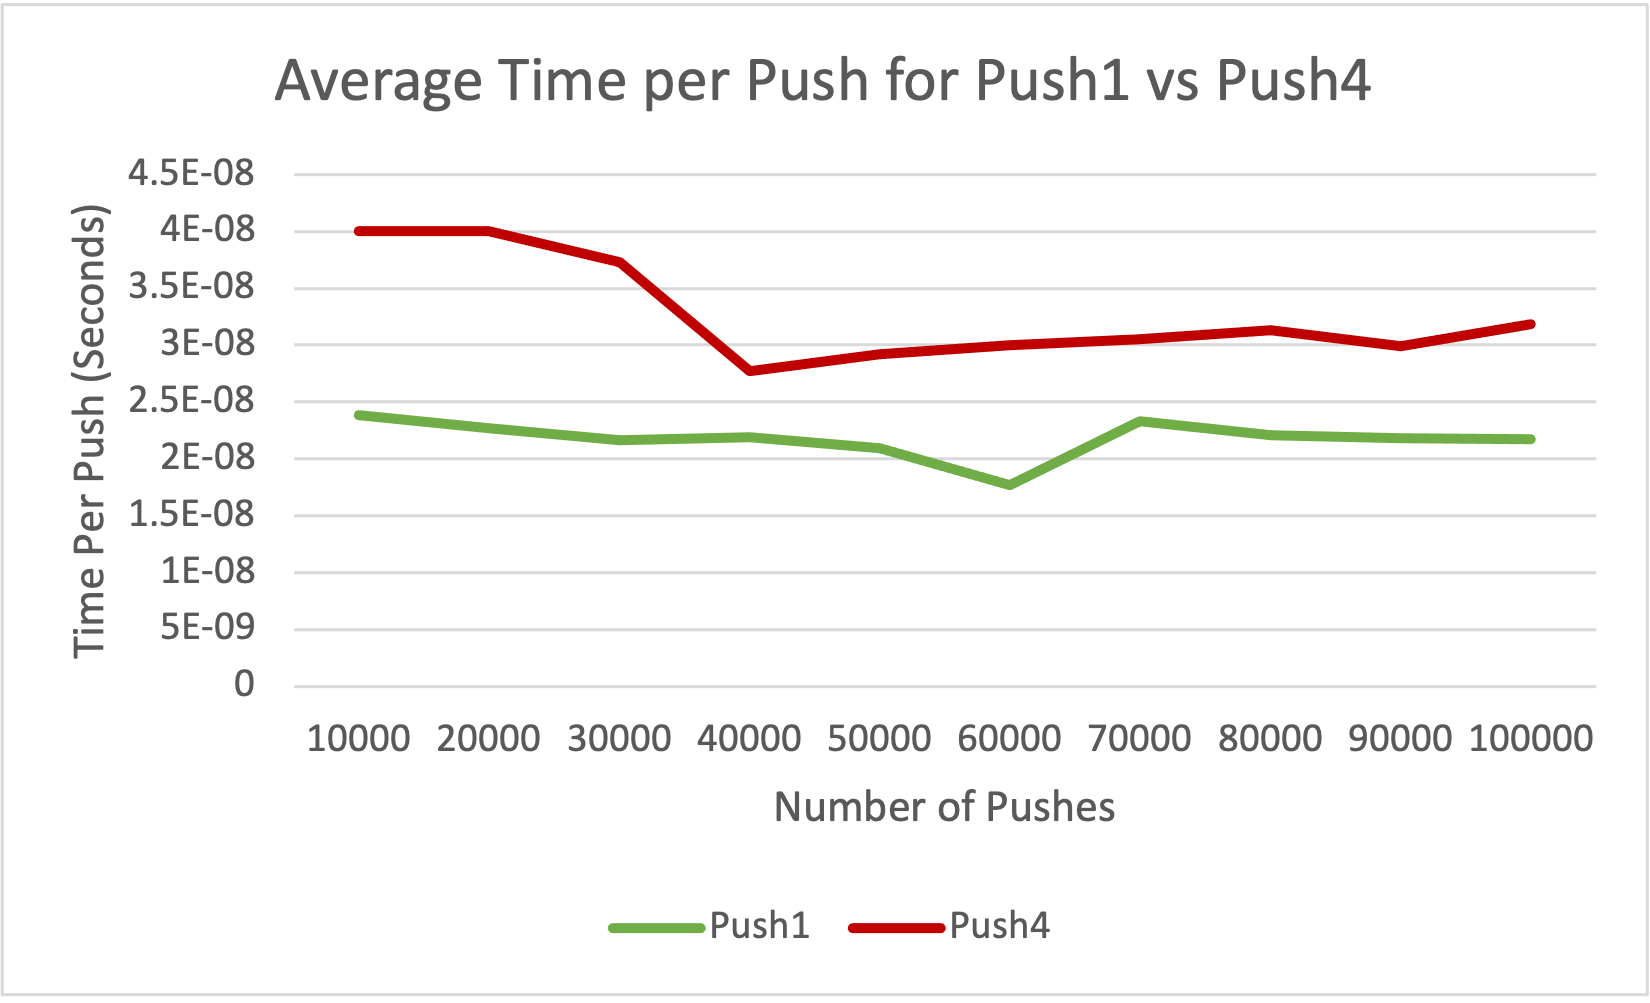
\includegraphics[width=\linewidth]{Figure3_0A.png}
  \caption{Average Time per Push for Push1 vs Push4}
  \label{fig:boat1}
\end{figure}

As seen in Figure 3, Push4 has similar efficiency to Push1, but is on average 1.041E-8 seconds slower per push than Push1. The time difference per push between Push4 and Push1 appears to vary, but Push4 never reaches the speed per push that Push1 does. This does not support the hypothesis that Push4 would be 0.5x slower than Push1.

\section{Part C: Data Structure Variations}

In order to implement a stack that stores multiple arrays, you would need to create an array of array pointers. You would also need to keep track of the size of each array within the array of pointers, the size of the array of array pointers, and the current index of the array that you are at. This way, when the current index is equal to the size, you can create a new pointer to a new array and put the new elements into it.  

\pagebreak

\subsection{Pseudocode for the push() function:}
if size of array == capacity:\\
    create new array w/ capacity * 2 within the array of pointers\\
    increment size, set equal to item\\
    
\subsection{Pseudocode for the top() function:}
pointer called Traverse that moves through the array of pointers,
increment Traverse until it is pointing to the last pointer in the array of array pointers, increment the last array pointer (A) that Traverse is currently pointing to until it is pointing to the last element in the last array within the array of pointers, dereference A\\

\subsection{Pseudocode for the pop() function:} 
pointer called Traverse that moves through the array of pointers\\
increment Traverse until it is pointing to the last pointer in the array of array pointers\\
decrement the size of the array that Traverse is pointing to\\

\subsection{Best case and worst case cost}
Best case cost: if array is empty, O(1)\\
Worst case cost: if array is full, O($n^2$)\\
This is worse than the original data structure cost (which is constant). As a function of n, the new data structure uses $n^2$ memory in the worst case (a.k.a. when the amount of empty space is at a maximum). The work required during a pop operation is $n^2$ (in terms of
array assignments). \\

\subsection{A pop algorithm that recovers memory as needed to bound the total memory usage}

Create an array of pointers and dereference them when you *pop* an element to bound total memory usage. As a function of the number of elements stored, this new data structure uses n memory in the worst case. The performance cost in terms of array copies of a pop in the worst case is n. The new algorithm does maintain a good average cost over all sequences of pushes and pops. 

\end{document}